\chapter{Optimization in Modern Machine Learning}
\label{Ch:OptimizationModernML}

\section{Adaptive Methods}
\label{Sec:Ada}

Adapted algorithms are those training algorithms that update the parameters 
under training using not only the current gradient information but also all past gradient information, as well as 
adaptively change the learning rate. These algorithms are sometimes also called to be belonging to the Ada--Series. 


\subsection{SGD with momentum}

Reference: Sutskever, I., Martens, J., Dahl, G., Hinton, G.,
On the importance and momentum in deep learning, \textit{ICML}, 2013.

\begin{algorithm}[H]
\caption{SGD with momentum ($=$ stochastic heavy ball method)}
\label{Alg:SGDMomentum}
\begin{algorithmic}[1]
\STATE \textbf{Input}: Input Initialization $w_0=w_{-1}$ and $v_{-1}=0$
\FOR {$k=0,1,...,K-1$}
    \STATE Randomly sample minibatch $\cS_i\subset\{1,2,...,n\}$ such that $|\cS_i|=m$
    \STATE Update $v_{k+1}=\mu v_k-\eta \dfrac{1}{m}\sum\li_{i\in \cS}\grad f_i(w_k)$
    \STATE Update $w_{k+1}=w_k+v_{k+1}$
\ENDFOR
\STATE \textbf{Output}: $w_K$
\end{algorithmic}
\end{algorithm}


\subsection{AdaGrad, RMSProp, AdaDelta}

Reference:

Duchi, J., Hazan, E., Singer, Y., Adaptive Subgradient Methods for Online Learning and
Stochastic Optimization, \textit{Journal of Machine Learning Research}, 2011, \textbf{12}(July), pp. 2121--2159.

AdaGrad not just accumulate historical information (such as square gradient information) but also adjust the learning rate 
(stepsize) according to the magnitude of historical gradient information at different dimensions, so that 
those dimensions with relatively small magnitudes of the gradient have larger learning rates. 
In this way, the algorithm favors some dimensions that have currently small magnitude of the gradient 
but contributes importantly to the optimization search path. This is more suitable to optimize 
neural network models that possess many local minimizers and saddle points. Empirical evidence shows that 
AdaGrad can stabilize SGD. The disadvantage of AdaGrad comes from the term $\sqrt{g_{k+1}}$
in the denominator, since as it accumulates during the training process the learning rates will gradually tend to $0$
and this leads to early stopping.

\begin{algorithm}[H]
\caption{AdaGrad}
\label{Alg:AdaGrad}
\begin{algorithmic}[1]
\STATE \textbf{Input}: Input Initialization $w_0$ and $g_0=0$
\FOR {$k=0,1,...,K-1$}
    \STATE Update $g_{k+1}=g_k+(\grad f(w_k))^2$
    \STATE Update $w_{k+1}=w_k-\dfrac{\eta \grad f(w_k)}{\sqrt{g_{k+1}}+\ve_0}$, $\ve_0>0$
\ENDFOR
\STATE \textbf{Output}: $w_K$
\end{algorithmic}
\end{algorithm}


Tieleman, T., Hinton, G., Lecture 6. 5--RmsProp: Divide the Gradient by A Running Average of its Recent Magnitude,
\textit{COURSERA, Neural Networks for Machine Learning}, 2012, \textbf{4}(2), pp. 26--31.

RMSProp is similar to AdaGrad but also makes use of the idea of SGD with momentum, this gives an 
exponential weight--decay average of historical information. RMSProp does a weighted average of both $g_k$
and $(\grad f(w_k))^2$, so that the weights in historical information will be small and thus it favors more on
current gradient information. This avoids the monotonic decay of the learning rate (stepsize) along with the training process.

\begin{algorithm}[H]
\caption{RMSProp}
\label{Alg:RMSProp}
\begin{algorithmic}[1]
\STATE \textbf{Input}: Input Initialization $w_0$ and $g_0=0$
\FOR {$k=0,1,...,K-1$}
    \STATE Update $g_{k+1}=\gm g_k+(1-\gm)(\grad f(w_k))^2$
    \STATE Update $w_{k+1}=w_k-\dfrac{\eta \grad f(w_k)}{\sqrt{g_{k+1}}+\ve_0}$, $\ve_0>0$
\ENDFOR
\STATE \textbf{Output}: $w_K$
\end{algorithmic}
\end{algorithm}

Zeiler, M.D., AdaDelta: An Adaptive Learning Rate Method,
arXiv:1212.5701, 2012.

AdaDelta, based on RMSProp, adjust the accumulated historical information according to the magnitude of gradients.

\begin{algorithm}[H]
\caption{AdaDelta}
\label{Alg:AdaDelta}
\begin{algorithmic}[1]
\STATE \textbf{Input}: Input Initialization $w_0$ and $u_0=0$, $v_0=0$ and $g_0=0$
\FOR {$k=0,1,...,K-1$}
    \STATE Update $g_{k+1}=\gm g_k+(1-\gm)(\grad f(w_k))^2$
    \STATE Update $v_{k+1}=\gm v_k+(1-\gm)u_k^2$
    \STATE Update $u_{k+1}=-\dfrac{\sqrt{v_k+\ve_0}\grad f(w_k)}{\sqrt{g_{k+1}}+\ve_0}$
    \STATE Update $w_{k+1}=w_k+u_{k+1}$
\ENDFOR
\STATE \textbf{Output}: $w_K$
\end{algorithmic}
\end{algorithm}

\subsection{Adam}

Reference:

Kingma, D.P., Ba, J.L., ADAM: A method for stochastic optimization,
\textit{ICLR}, 2015.

Reddi, S.J., Kale, S., Kumar, S., On the convergence of ADAM and Beyond,
\textit{ICLR}, 2018.

Adam combines all ingredients in SGD--momentum, AdaGrad, RMSProp, AdaDelta: 
(1) The update direction is determined by accumulated historical gradient information;
(2) Correct the stepsize using accumulated square gradient information;
(3) Exponential decay of accumulated information. Adam has been widely used in training neural networks.

\begin{algorithm}[H]
\caption{Adam}
\label{Alg:Adam}
\begin{algorithmic}[1]
\STATE \textbf{Input}: $\al$: stepsize; $\bt_1, \bt_2\in [0,1)$: Exponential decay rates for the moment estimates;
                        $f(\tht)$: stochastic objective function with parameters $\tht$;
                        $\tht_0$: initial parameter vector; $m_0 \leftarrow 0$ (initialize first moment vector);
                        $v_0 \leftarrow 0$ (initialize second moment vector);
                        $t \leftarrow 0$ (initialize timestep)
\WHILE {$\tht_t$ not converged}
    \STATE $t \leftarrow t+1$
    \STATE $g_t \leftarrow \grad_\tht f_t(\tht_{t-1})$ (Get gradients w.r.t. stochastic objective at timestep $t$)
    \STATE $m_t \leftarrow \bt_1\cdot m_{t-1}+(1-\bt_1)\cdot g_t$ (Update biased first moment estimate)
    \STATE $v_t \leftarrow \bt_2\cdot v_{t-1}+(1-\bt_2)\cdot g_t^2$ (Update biased second raw moment estimate)
    \STATE $\hat{m}_t \leftarrow m_t/(1-\bt_1^t)$ (Compute bias--corrected first moment estimate)
    \STATE $\hat{v}_t \leftarrow v_t/(1-\bt_2^t)$ (Compute bias--corrected second raw moment estimate)
    \STATE $\tht_t \leftarrow \tht_{t-1}-\al\cdot \hat{m}_t/(\sqrt{\hat{v}_t}+\ve)$ (Update parameters)
\ENDWHILE
\STATE \textbf{Output}: $\tht_t$ (Resulting parameters)
\end{algorithmic}
\end{algorithm}

\section{Training a Transformer: AdamW and Muon}
\label{Sec:Transformer}

\subsection{Transformer Neural Network}

GPT uses transformer network so we take this example. 

\noindent{\textbf{Computational Modules.}}

$\bullet$ RMS norm: normalization of token's embedding vector $\boldx \in \R^d$. There are no learnable params in RMSNorm. This is different from transformer paper's LayerNorm.

$$\text{RMSNorm}(\boldx)=\dfrac{\boldx}{\text{RMS}(\boldx)+\ve} \ , \ \text{RMS}(\boldx)=\sqrt{\sum\li_{i=1}^d x_i^2} \ , \ \boldx = (x_1,...,x_d) \ , \ \ve>0 \ .$$

\

$\bullet$ Rotary Positional Embedding (RoPE): positional embedding using $\sin$, $\cos$ positional tensors. This is different from transformer paper's Positional Embedding.

Input $x$ (which is the $Q,K$ in causal attention module) with shape $(B, T, H, D)$ where  $B=$batch size, $T=$sequence length, $H=$number of heads in multi-head attention, $D=$dimension of each head (must be even). Let $\sin=(\sin^{t,i})_{0\leq t \leq T-1, 0\leq i\leq D/2}$, $\cos=(\cos^{t,i})_{0\leq t \leq T-1, 0\leq i\leq D/2}$ be tensors each with shape $(1,T,1,D/2)$. Then for each batch $b$, each index $t\in \{0,...,T-1\}$, each head $h$, RoPE does the following:
$$(x^{b,t,h,0},...,x^{b,t,h,D-1}) \ra \left\{\begin{array}{ll}
\cos^{t,i}x^{b,t,h,i} + \sin^{t,i}x^{b,t,h,i+D/2} & \text{ for } 0\leq i \leq D/2-1 \ ,
\\
-\sin^{t,i-D/2}x^{b,t,h,i-D/2} + \cos^{t,i-D/2}x^{b,t,h,i} & \text{ for } D/2\leq i \leq D-1 \ .
\end{array}\right.$$
Position information, originally in $t$, is encoded in such rotation via $\cos, \sin$. Usually we take $\cos^{t,i}=\cos \left(\dfrac{t}{10000^{2i/D}}\right)$ and $\sin^{t,i}=\sin \left(\dfrac{t}{10000^{2i/D}}\right)$.

\

$\bullet$ Causal Self-Attention. The self-attention module with specific causal mask construction.

-- number of heads $\verb#n_head#$ $\%$ number of kv heads $\verb#n_kv_head#$ $=0$. 

-- self-attention. Input $x$ has shape $(B,T,\verb#_#)$, which stands for the current forward pass. Then $Q, K, V$ are from input $x$, i.e., $Q=W_Q^T X$ etc. They are re-shaped into shape $(B,T, \verb#n_head#, \verb#head_dim#)$ for $Q$ and $(B,T, \verb#n_kv_head#, \verb#head_dim#)$ for $K, V$, respectively. 
Then apply RoPE to $Q,K$, apply RMSNorm to $Q,K$, finally apply $(1,2)$ transpose $(B,T,H,D)\ra (B,H,T,D)$ to $Q,K,V$, i.e., to process each attention head to the full batch (head-wise parallelization);

-- kv-cache and multi-query-attention. $T$ in $(B,H,T,D)$ stands for the number of queries. For $Q$, use number of queries in this forward pass $=T_q$; for $K,V$, after kv-cache, use number of queries in the cache $+$ current forward pass $=T_q+(T_k)_{\text{prev}}=T_k$.

PyTorch 2.0's \verb`scaled_product_attention`: 

\begin{verbatim}
def scaled_dot_product_attention(
    query: Tensor,
    key: Tensor,
    value: Tensor,
    attn_mask: Tensor | None = None,
    dropout_p: float = 0.0,
    is_causal: bool = False,
    scale: float | None = None,
    enable_gqa: bool = False,
) -> Tensor: ...
\end{verbatim}

Multi-Query-Attention (Group-Query-Attention, gqa): 

\verb#enable_gqa = self.n_head != self.n_kv_head#:
multiple query heads use the same key/value head, or in other words duplicately use key/value head for a chunk of query heads. This saves computation. Example: \verb#n_head#$=16$, \verb#n_kv_head#$=4$, then each group of $4$ query heads share the same kv head, or the same kv head repeatedly used $4$ times for each chunk of $4$ query heads. 

Mask construction in multi-query-attention: Discuss the following cases
\begin{itemize}
\item[(1)] Inference with no increment, i.e. infer the whole sequence at once ($T_q=T_k$) or training (kv cache is empty): Auto regressive case. Each query only attends keys/values before it. Use standard causal mask. See Figure \ref{Fig:MQAmasks} left. 
\item[(2)] $T_q=1$, inference with single query in this forward pass. Each query attends all the keys/values in the cache. No mask needed. See Figure \ref{Fig:MQAmasks} middle.
\item[(3)] Not (1) or (2): $1<T_q<T_k$. Inference with a chunk of $T_q$ queries in this forward pass. Each query attends all the keys/values in the old kv cache $(T_k)_\text{prev}=T_k-T_q$, but for the newly added $T_q$ items of kv, i.e. within the chunk we use causal attention so that each query only attends keys/values before it. See Figure \ref{Fig:MQAmasks} right.
\end{itemize}

\begin{figure}[H]
\centering
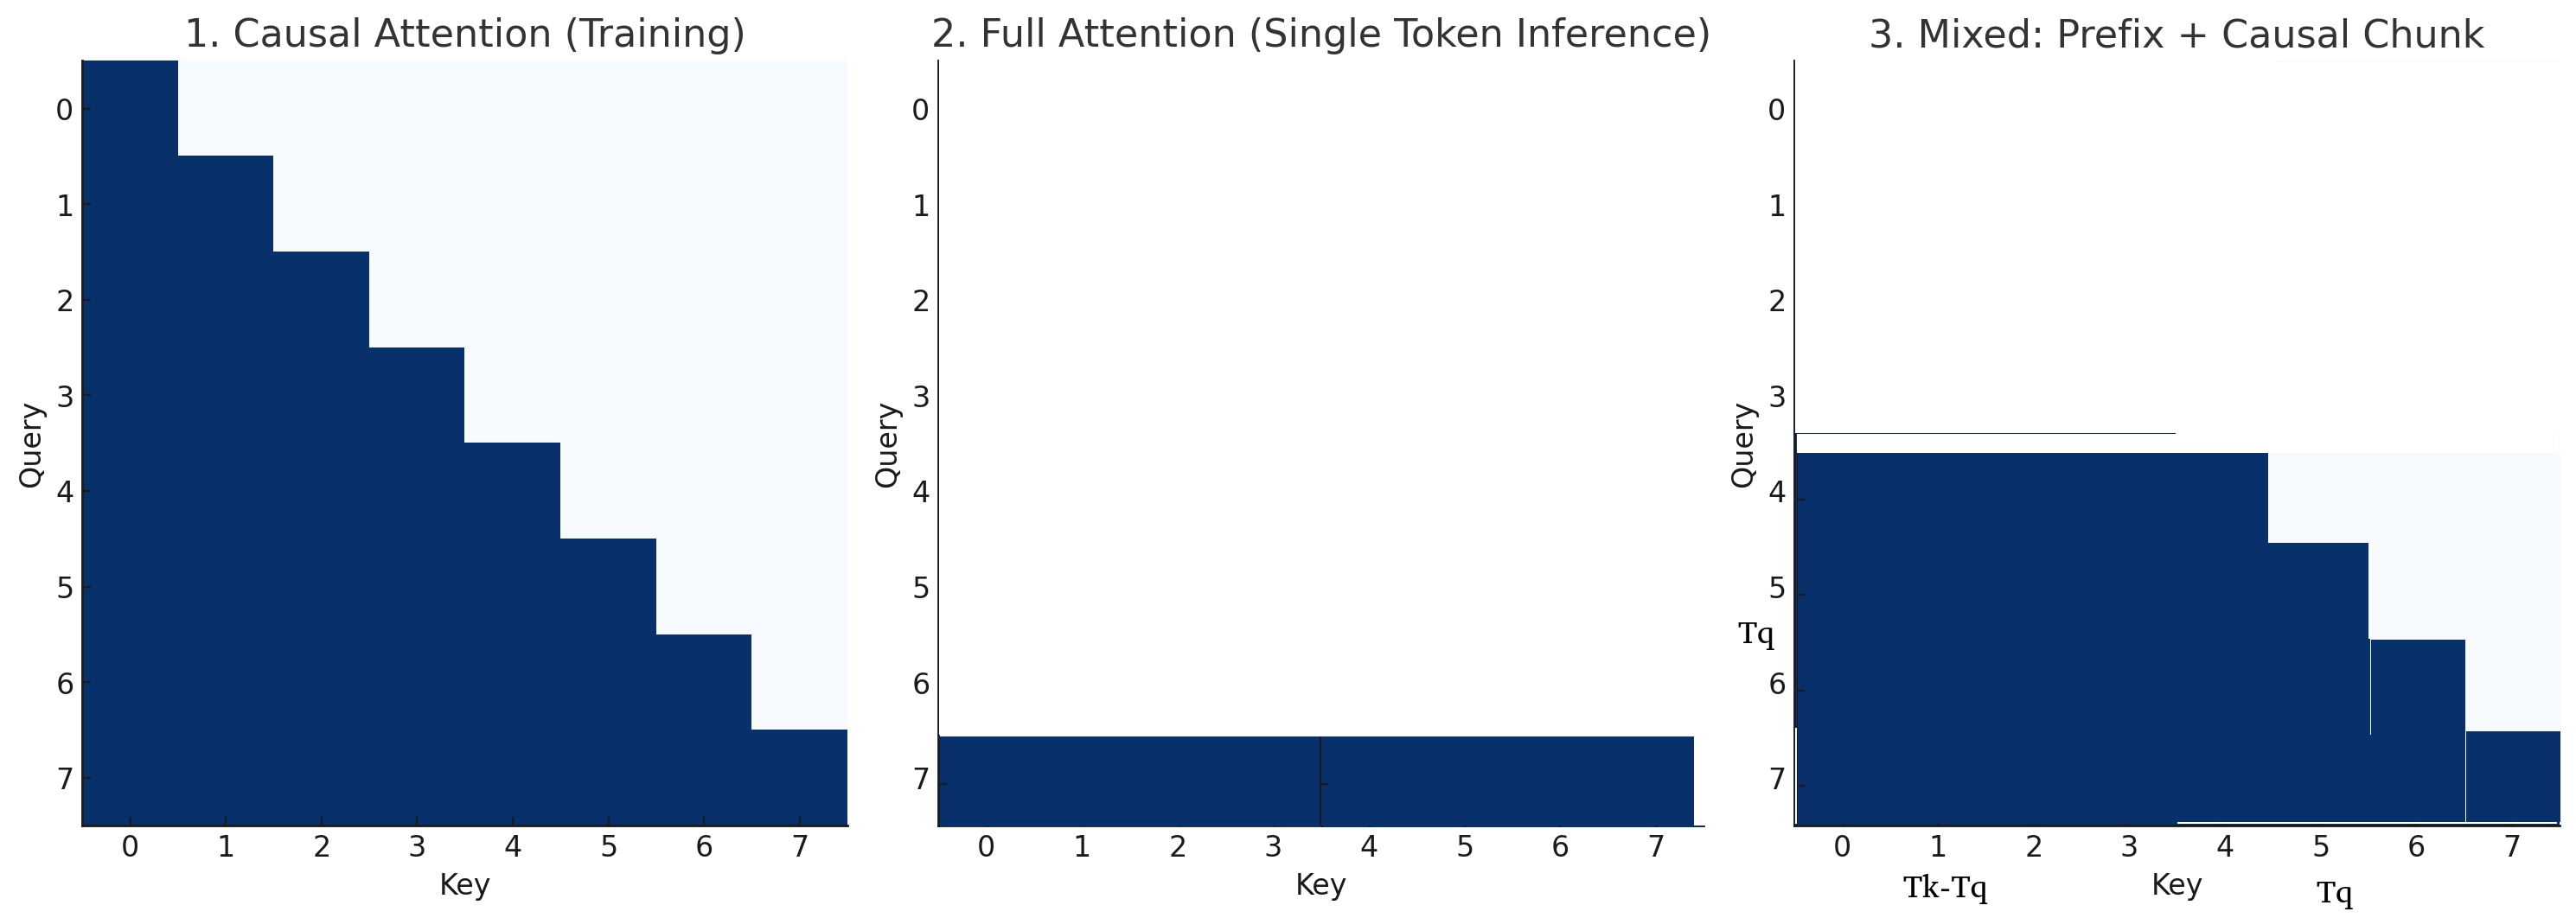
\includegraphics[height=5.2cm, width=15cm]{figures/Fig_MQAmasks.png}
\caption{MQA masks.}
\label{Fig:MQAmasks}
\end{figure}

-- final projection. Concatenate heads $$(B,\verb#n_head#, T, \verb#head_dim#)\ra (B, T, \verb#n_head#, \verb#head_dim#)\ra (B, T, \verb#n_head#\times \verb#head_dim#) \ .$$ Followed by a linear layer $\verb#n_head#\times \verb#head_dim# \ra \verb#n_embd#$.

$\bullet$ MLP. Layer structure: \verb#n_embd# $\ra$ $4\times$ \verb#n_embd# $\stackrel{\text{ReLU}^2}{\longrightarrow}$ \verb#n_embd#. Activation function use $$\text{ReLU}^2(x)=\left\{\begin{array}{ll}
x^2 & \text{ if } x\geq 0 \ , 
\\
0 & \text{ if } x<0 \ .
\end{array}
\right.$$

$\bullet$ Block. Use residual connections $$x\mapsto x'=x+\text{Causal Self-Attention}\mapsto x'' = x'+\text{MLP} \ .$$

\noindent{\textbf{The whole GPT workflow.}}

$\bullet$ Network architecture: 

-- \verb#wte#: word-to-embedding layer, \verb#vocab_size#$=50304$ is the amount of tokens, \verb#n_embd#$=768$ is the embedding dimension.

-- \verb#h#: transformer block layer, \verb#n_layer#$=12$ layers of Block.

-- \verb#lm_head#: language modeling head, head layer, embedding $\ra$ token logits (\verb#vocab_size# tokens).

\begin{verbatim}
Input ids
   ↓
Embedding (wte)
   ↓
Norm
   ↓
n_layer × Transformer Blocks (Block) (n_layer=12)
   ↓
Norm
   ↓
Linear Output Head (lm_head)
   ↓
Logits / Loss
\end{verbatim}

$\bullet$ Initialize weights:

-- linear layers: $\cN(0, \sm)$ where $\sm=\dfrac{1}{\sqrt{fan\_in}}\cdot \left(1\wedge \sqrt{\dfrac{fan\_out}{fan\_in}}\right)$

-- embedding layers: $\cN(0,1)$

-- \verb#lm_head# weights: 0

-- \verb#c_proj# weights: 0

-- initialize the rotary embeddings: \verb#_precompute_rotary_embeddings()#, use $\cos^{t,i}=\cos \left(\dfrac{t}{10000^{2i/D}}\right)$ and $\sin^{t,i}=\sin \left(\dfrac{t}{10000^{2i/D}}\right)$ as we indicated before, with \verb#rotary_seq_len#, i.e. running range of $t$, being $10$ times of the \verb#seq_len#$=1024$.

$\bullet$ Optimizers: AdamW for embedding layers and Muon for linear layers.

$\bullet$ Computing the logits: \verb#lm_head# layer, softcap the logits using $15*$\verb#tanh#$\left(\dfrac{\text{logit}}{15}\right)$ (\verb#softcap#$=15$). Training mode use cross-entropy loss towards the \verb#target#.

$\bullet$ Naive autoregressive streaming inference: generate the next token through output logits. Only first top $k$ logits are considered before softmax. Then softmax logits with control of randomness using \verb#tempreature#: when \verb#tempreature#$>0$, then $\dfrac{\text{logit}}{\text{tempreature}}$ as the new \verb#logit#, then softmax and random sampling; but when \verb#tempreature#$=0$, deterministically sample argmax of \verb#logit#.

$\bullet$ Use of \verb#bfloat16# for GPU. 

\subsection{AdamW}

\subsection{Muon}

\section{Dual Methods}
\label{Sec:Dual}

\subsection{Dual Coordinate Descent/Ascent}

Reference: Chapter 13 \& 14 of Nocedal, J., Wright, S.J., \textit{Numerical Optimization}, Second Edition, Springer, 2006.

Constraint optimization problem $P_0$:

$$\begin{array}{c}
\min\li_{w}f(w) \\
\text{s.t. } g_i(w)\leq 0 \ , \ i=1,2,...,m_1 \ , \
h_j(w)=0 \ , \ j=1,2,...,m_2  \ . \\
\end{array}$$
Let the optimal solution be $p^*$.

Unconstrained Version:
$$\min\li_{w}\left(f(w)+\infty\sum\li_{i=1}^{m_1}\One_{[g_i(w)>0]}+\infty\sum\li_{j=1}^{m_2}\One_{[h_j(w)\neq 0]}\right) \ .$$

Approximate the indicators by linear functions, obtain the Lagrangian function

$$L(w,\lb,\nu)\equiv f(w)+\sum\li_{i=1}^{m_1}\lb_i g_i(w)+\sum\li_{j=1}^{m_2}\nu_j h_j(w)  \ ,$$
in which $\lb_i\geq 0$ and $\nu_j\in \R$ are the \textit{Lagrange multipliers}. The variable $w$ is called the \textit{primal} variable.

Set the \textit{Lagrangian dual function}
$$h(\lb, \nu)\equiv \inf\li_{\text{acceptable } w}L(w,\lb,\nu) \ , \ \lb_i\geq 0 \text{ and } \nu_j\in \R \ .$$
Since for any acceptable $w$ we have $g_i(w)\leq 0$ and $h_i(w)=0$, so we have
$$h(\lb, \nu)\leq \inf\li_{\text{acceptable } w}f(w)=p^* \ .$$

The variables $(\lb, \nu)$ are called \textit{dual} variables. 

Observation: $h(\lb, \nu)$ is always concave (even when the original problem $P_0$ is not convex) in the dual variables $\lb$ and $\nu$.

Dual Problem $D_0$ (``primal-dual"):

$$\begin{array}{c}
\max\li_{\lb, \nu}h(\lb, \nu) \\
\text{s.t. }  \lb_i\geq 0 \ , \ i=1,2,...,m \ .
\end{array}$$
Let the optimal solution be $d^*$. Then $d^*\leq p^*$.

If $d^*=p^*$ this is called \textit{strong duality}. A sufficient condition for strong duality is Slater condition and
a necessary condition for strong duality is KKT condition.

Set $d^*=h(\lb^*, \nu^*)$. Then solve the unconstrained optimization problem
$$\min\li_{w}L(w,\lb^*, \nu^*) \ .$$
If the solution is acceptable then it is the optimal solution for the original problem.

\begin{algorithm}[H]
\caption{Dual Coordinate Ascent}
\label{Alg:DualCoordinateAscent}
\begin{algorithmic}[1]
\STATE \textbf{Input}: Input Initialization $v_0$, $\lb_0\geq 0$
\FOR {$k=0,1,...,K-1$}
    \STATE Calculate $w_k$ such that $w_k=\arg\min\li_{w}L(w,\lb_{k-1},v_{k-1})$
    \STATE Update $\lb_{k,i}=\max\{\lb_{k-1,i}+\eta_k g_i(w_k), 0\}$, $i=1,2,...,m_1$
    \STATE Update $v_{k,j}=v_{k-1,j}+\eta_k h_j(w_k)$, $j=1,2,...,m_2$
\ENDFOR
\STATE \textbf{Output}: $w_K$
\end{algorithmic}
\end{algorithm}


\subsection{SDCA}

Shalev--Schwarz, S., Zhang, T., Stochastic Dual Coordinate Ascent Methods for Regularized Loss Minimization,
\textit{Journal of Machine Learning Research}, \textbf{14}(2013), pp. 567--599.

Let $x_1,...,x_n$ be vectors in $\R^d$ and $\phi_1,...,\phi_n$ be a sequence of scalar convex functions, 
and let $\lb>0$ be a regularization parameter. Our goal is to solve the optimization problem 
$P(w^*)=\min\li_{w\in \R^d}P(w)$ where
$$P(w)=\dfrac{1}{n}\sum\li_{i=1}^n \phi_i(w^Tx_i)+\dfrac{\lb}{2}\|w\|^2 \ .$$ 

Here $\phi_i(w^Tx_i)$ is the loss function for linear models. 
For example, given labels $y_1,...,y_n$ in $\{\pm 1\}$, the SVM problem (with linear kernels and no bias term)
is obtained by setting $\phi_i(a)=\max\{0, 1-y_ia\}$; regularized logistic regression is obtained by setting 
$\phi_i(a)=\log(1+\exp(-y_ia))$; ridge regression is obtained by setting $\phi_i(a)=(a-y_i)^2$;
regression with the absolute--value is obtained by setting $\phi_i(a)=|a-y_i|$; support vector regression
is obtained by setting $\phi_i(a)=\max\{0, |a-y_i|-\nu\}$ for some predefined insensitivity parameter $\nu>0$.

Dual formulation: $D(\al^*)=\max\li_{\al\in \R^d}D(\al)$ where

$$D(\al)=\dfrac{1}{n}\sum\li_{i=1}^n -\phi_i^*(-\al_i)
-\dfrac{\lb}{2}\left\|\dfrac{1}{\lb n}\sum\li_{i=1}^n \al_ix_i\right\|^2$$
where $\phi_i^*(u)=\max\li_{z}(zu-\phi_i(z))$. 

In fact we have

$$\begin{array}{ll}
\min\li_w P(w) & =\min\li_w \left[\dfrac{1}{n}\sum\li_{i=1}^n (\phi_i(w^T x_i)+\al_i(w^Tx_i))+\dfrac{\lb }{2}\left(\|w\|^2-\dfrac{2}{\lb n}\sum\li_{i=1}^n \al_iw^Tx_i\right)\right]
\\
& =\min\li_w \left[\dfrac{1}{n}\sum\li_{i=1}^n (\phi_i(w^T x_i)+\al_i(w^Tx_i))+\dfrac{\lb }{2}\left\|w-\dfrac{1}{\lb n}\sum\li_{i=1}^n \al_i x_i\right\|^2-\dfrac{\lb}{2}\left\|\dfrac{1}{\lb n}\sum\li_{i=1}^n \al_i x_i\right\|^2\right]
\\
& \geq \min\li_w \left[\dfrac{1}{n}\sum\li_{i=1}^n (\phi_i(w^T x_i)+\al_i(w^Tx_i))\right]-\dfrac{\lb}{2}\left\|\dfrac{1}{\lb n}\sum\li_{i=1}^n \al_i x_i\right\|^2
\\
& \geq \dfrac{1}{n}\sum\li_{i=1}^n \min\li_{\om}(\phi_i(w^T x_i)+\al_i(w^Tx_i))-\dfrac{\lb}{2}\left\|\dfrac{1}{\lb n}\sum\li_{i=1}^n \al_i x_i\right\|^2
\\
& \geq \dfrac{1}{n}\sum\li_{i=1}^n -\max\li_{z}(-\phi_i(z)-\al_iz)-\dfrac{\lb}{2}\left\|\dfrac{1}{\lb n}\sum\li_{i=1}^n \al_i x_i\right\|^2
\\
& = \dfrac{1}{n}\sum\li_{i=1}^n -\phi_i^*(-\al_i)-\dfrac{\lb}{2}\left\|\dfrac{1}{\lb n}\sum\li_{i=1}^n \al_i x_i\right\|^2=D(\al)
\end{array}$$
for any $\al\in \R^d$. 

So $\min\li_w P(w)\geq \max\li_\al D(\al)$. Set $w(\al)=\dfrac{1}{\lb n}\sum\li_{i=1}^n \al_i x_i$, then strong duality holds and 

$$w(\al^*)=w^* \ , \ P(w^*)=D(\al^*) \ .$$

\begin{algorithm}[H]
\caption{Stochastic Dual Coordinate Ascent}
\label{Alg:SDCA}
\begin{algorithmic}[1]
\STATE \textbf{Input}: Input Initialization $\al_0$, $w_0=w(\al_0)$
\FOR {$k=0,1,...,K-1$}
    \STATE Randomly sample $i_k\in \{1,2,...,n\}$
    \STATE Find $\Dt \al_{i_k}=\arg\max\li_{z}\left\{-\phi_{i_k}^*(-\al_{k,i}+z)
                -\dfrac{\lb n}{2}\left\|w_k+\dfrac{1}{\lb n}zx_{i_k}\right\|^2\right\}$
    \STATE Update $\al_{k+1}=\al_k+\Dt \al_{i_k}e_{i_k} \ , \ w_{k+1}=w_k+\dfrac{1}{\lb n}\Dt \al_{i_k}x_{i_k}$
\ENDFOR
\STATE \textbf{Output (Average Option)}: $\bar{\al}=\dfrac{1}{K-K_0}\sum\li_{i=K_0+1}^K \al_{i}$ and 
                $\bar{w}=w(\bar{\al})=\dfrac{1}{K-K_0}\sum\li_{i=K_0+1}^K w_{k-1}$, return $\bar{w}$
\STATE \textbf{Output (Random Option)}:  Let $\bar{\al}=\al_k$ and $\bar{w}=w_k$ for some random $k\in K_0+1,...,K$, return $\bar{w}$
\end{algorithmic}
\end{algorithm}

\section{Optimization with Constraints and Discontinuous Objective Function}
\label{Sec:ConstraintAndDiscontinuousOptimization}

\subsection{Subgradient Projection Method, Frank--Wolfe Method}

References:

Levitin, E.S., Polyak, B.T., Constrained Minimization Methods, \textit{USSR Computational Mathematics and Mathematical Physics},
1966, \textbf{6}(5), pp. 1--50.

Frank, M., Wolfe, P., An algorithm for quadratic programming, \textit{Naval Research Logistics (NRL)}, 1956, \textbf{3}(1--2), pp. 95--110.

\

The subgradient $\pt f(x_0)$ for a convex function at point $x_0$ is defined as
$$\pt f(x_0)=\{c\in \R: f(x)-f(x_0)\geq c(x-x_0) \} \ . $$

\begin{algorithm}[H]
\caption{Subgradient Projection Method}
\label{Alg:SubgradientProjection}
\begin{algorithmic}[1]
\STATE \textbf{Input}: Input Initialization $x_0$; Convex Set $\cX$; learning rate $\eta>0$
\FOR {$k=0,1,...,K-1$}
    \STATE Randomly sample a subgradient $g_k\in \pt f(x_k)$
    \STATE Update $y_{k+1}=x_k-\eta g_k$
    \STATE Project $x_{k+1}=\Pi_{\cX} (y_{k+1})$, $\Pi_{\cX}(y)=\arg\min\li_{x\in \cX}\|y-x\|$
\ENDFOR
\STATE \textbf{Output}: $x_K$
\end{algorithmic}
\end{algorithm}

The projection $\Pi_{\cX}(y)$ can be hard to calculate in practical cases.
However, subgradient projection $=$ first gradient descent then projection;
Frank--Wolfe $=$ combine gradient descent with projection to constraint.

How to do that? GD is an optimal choice of search direction via first--order Taylor expansion:
$$f(x+td)=f(x)+t\grad f(x+\gm td)^Td \text{ for some } \gm\in (0,1) \ .$$

If $d^T\grad f(x)<0$, then $d$ is a descent direction.

``Steepest Descent": $d_{\text{optimal}}=\arg\inf\li_{\|d\|=1}d^T \grad f(x)=-\dfrac{\grad f(x)}{\|\grad f(x)\|}$.

Want to incorporate the constraint information: how to do that?

$$d_{\text{optimal}}=\arg\inf\li_{d\in \cX}d^T \grad f(x) \ .$$

\begin{algorithm}[H]
\caption{Frank--Wolfe Method}
\label{Alg:Frank-Wolfe}
\begin{algorithmic}[1]
\STATE \textbf{Input}: Input Initialization $x_0\in \cX$; Convex Set $\cX$; weights $\eta_k>0$
\FOR {$k=0,1,...,K-1$}
    \STATE Calculate $\grad f(x_k)$
    \STATE Update $d_k=\arg\inf\li_{d\in \cX}d^T\grad f(x_k)$
    \STATE Update $x_{k+1}=(1-\gm_k)x_k+\gm_k d_k$
\ENDFOR
\STATE \textbf{Output}: $x_K$
\end{algorithmic}
\end{algorithm}

\subsection{ADMM}

Reference: Boyd, S., Parikh, N., Chu, E., Peleato, B., Eckstein, J.,
Distributed Optimization and Statistical Learning via the Alternating Direction Method of Multipliers,
\textit{Foundations and Trends in Machine Learning}, Vol. 3, No. 1 (2010), pp. 1--122.

\

Equality--constrained convex optimization problem:
$$\text{minimize } f(x) \text{ subject to } Ax=b \ .$$

\underline{Augmented Lagrangian}. 

$$L_{\rho}(x,y)=f(x)+y^T(Ax-b)+\dfrac{\rho}{2}\|Ax-b\|_2^2 \ .$$

The augmented Lagrangian can be viewed as the (unaugmented) Lagrangian associated 
with the problem
$$\text{minimize } f(x)+\dfrac{\rho}{2}\|Ax-b\|_2^2 \text{ subject to } Ax=b \ .$$

This problem can be solved by dual gradient ascent: 

$$\begin{array}{lll}
x^{k+1} & \equiv & \arg\min\li_{x} L(x, y^k) \ , \\
y^{k+1} & \equiv & y^k+\rho (Ax^{k+1}-b) \ .
\end{array}$$


\

\underline{Alternating Direction Method of Multipliers (ADMM)}.

\

Optimization problem has the form
$$\text{minimize } f(x)+g(z) \text{ subject to } Ax+Bz=c \ .$$

Optimal value 
$$p^*=\inf\{f(x)+g(z); Ax+Bz=c\} \ .$$

Augmented Lagrangian can be formed as 

$$L_{\rho}(x,z,y)=f(x)+g(z)+y^T(Ax+Bz-c)+\dfrac{\rho}{2}\|Ax+Bz-c\|_2^2 \ .$$

This problem can be solved by dual gradient ascent: 

$$\begin{array}{lll}
(x^{k+1}, z^{k+1}) & \equiv & \arg\min\li_{x,z}L_{\rho}(x,z,y^k) \ , \\
y^{k+1} & \equiv & y^k+\rho(A x^{k+1}+B z^{k+1}-c) \ .
\end{array}$$

Unlike the classical dual gradient ascent which minimizes the augmented Lagrangian jointly with respect to 
the two primal variables $x$ and $z$, ADMM updates $x$ and $z$ in an alternating or sequential fashion, which accounts 
for the term \textit{alternating direction}.  

\begin{algorithm}[H]
\caption{Alternating Direction Method of Multipliers}
\label{Alg:ADMM}
\begin{algorithmic}[1]
\STATE \textbf{Input}: Input Initialization $(x^0, z^0)$, dual variable $y^0$, parameter $\rho>0$
\FOR {$k=0,1,...,K-1$}
    \STATE Calculate $x^{k+1}\equiv \arg\min\li_{x} L_{\rho}(x, z^k, y^k)$
    \STATE Calculate $z^{k+1}\equiv \arg\min\li_{z} L_{\rho}(x^{k+1}, z, y^k)$
    \STATE Calculate $y^{k+1}=y^k+\rho(Ax^{k+1}+Bz^{k+1}-c)$
\ENDFOR
\STATE \textbf{Output}: $(x^K, z^K)$
\end{algorithmic}
\end{algorithm}

\subsection{Proximal operators and proximal algorithms}

Reference: Parikh, N., Boyd, S., Proximal Algorithms, \textit{Foundations and Trends in Optimization},
Vol. 1, No. 3 (2013), pp. 123--231.

Also see \url{http://stanford.edu/~boyd/papers/pdf/prox_slides.pdf}

Let $R=R(v)$ be a convex function. With respect to the convex function $R$ 
the proximal operator $\text{prox}_R(w): \R^d\ra \R^d$ is defined as 
$$\text{prox}_R(w)=\arg\min\li_{v}\left(R(v)+\dfrac{1}{2}\|w-v\|^2\right) \ .$$

If $R(w)=0$, then $\text{prox}_0(w)=w$; if $R(w)=aI_C(w)$ (where $C\subseteq \R^d$ is usually a convex set, and the indicator function is defined as in \eqref{Eq:Indicator}), then $\text{prox}_{a I_C}(w)=\arg\min\li_{v\in C}\|w-v\|^2$
degenerates to a projection operator. 

We have 
$$p=\text{prox}_R(w) \Longleftrightarrow w-p\in \pt R(p) \ .$$
Also
$$\text{prox}_{aR}(w)=\arg\min\li_v\left(R(v)+\dfrac{1}{2a}\|w-v\|^2\right) \ .$$

Convex optimization problem
$$\min\li_{w\in \cW} f(w)=l(w)+R(w) \ ,$$
where $l(w)$ is a convex differentiable function and $R(w)$ is non--differentiable convex function (such as $L_1$--regularization term).

\begin{algorithm}[H]
\caption{Proximal Gradient Descent}
\label{Alg:ProximalGD}
\begin{algorithmic}[1]
\STATE \textbf{Input}: Input Initialization $w_0$, convex set $\cW$, learning rates $\eta_k>0$
\FOR {$k=0,1,...,K-1$}
    \STATE Calculate $\grad l(w_k)$
    \STATE Update parameter $v_{k+1}=w_k-\eta_k \grad l(w_k)$
    \STATE Apply proximal operator $w_{k+1}=\text{prox}_{\eta_k R}(v_{k+1})$
\ENDFOR
\STATE \textbf{Output}: $w_K$
\end{algorithmic}
\end{algorithm}

\section{Optimization and Generalization}
\label{Sec:OptimizationAndGeneralization}

\subsection{Generalization Bounds in Statistical Machine Learning}

Consider the supervised learning framework. Let the training sample
$(x_1, y_1)$, $...$, $(x_N, y_N)$ follow the same distribution $(x,y)\sim F(x,y)$ under probability measure $\Prob$
(or $\Prob_{(x,y)}$, and the corresponding expectation is $\E$ or $\E_{(x,y)}$).
Let the loss functions be
$\ell_i(\theta)=\ell((x_i, y_i), \theta)$, $\theta\in \mathbb{R}^d$, $i=1,2,...,N$.
Define the empirical loss function

\begin{equation}\label{Eq:EmpiricalLossFunction}
L_N(\tht)=\dfrac{1}{N}\sum\li_{i=1}^N \ell_i(\tht) \ .
\end{equation}

Let the local minimizer of $L_N(\tht)$ be $\tht^*_N$, which may not be unique (in this case we
further denote them as $\tht_N^{*,1}, ..., \tht_N^{*,k}$).
Then the empirical loss function evaluated at $\tht_N^*$
is $L_N(\tht_N^*)$. The \textit{generalization gap} is defined to be

\begin{equation}\label{Eq:GeneralizationGap}
\text{Gap}_N  \equiv \left|L_N(\tht_N^*)-\E_{(x,y)} \ell((x,y), \tht_N^*)\right|
= \left|\dfrac{1}{N}\sum\li_{i=1}^N \ell((x_i, y_i), \tht_N^*)-\E_{(x,y)} \ell((x,y), \tht_N^*)\right| \ .
\end{equation}

We further define the \textit{two-sided generalization gaps} as

\begin{equation}\label{Eq:GeneralizationGap-Empirical-Expected}
\text{Gap}_N^+  \equiv L_N(\tht_N^*)-\E_{(x,y)} \ell((x,y), \tht_N^*) \ ,
\end{equation}

\begin{equation}\label{Eq:GeneralizationGap-Expected-Empirical}
\text{Gap}_N^-  \equiv \E_{(x,y)} \ell((x,y), \tht_N^*)-L_N(\tht_N^*) \ .
\end{equation}


In classical statistical learning theory, the basic estimates of generalization gap
bounds \footnote{see Vapnik, V., \textit{Statistical Learning Theory}, Wiley-Interscience, first edition, 1988.}
are bounding $\text{Gap}_N$
in \eqref{Eq:GeneralizationGap} in terms of features of the family of functions
that consists of the loss functions $\ell_i(\tht)$ in which we vary the parameters $\tht$ and
the training data points $(x_i, y_i)$, $i=1,2,...,N$.
Typical such features are the \textit{Vapnik-Chervonenkis dimension} (VC dimension) and
the \textit{Rademacher complexity}. 

(a) VC dimension. Let the loss function be $\ell((x,y), \tht)=\One(h(x,\tht)\neq y)$ for a family of functions $h(x,\tht)$, $\tht\in \Tht$.
Then we define the \textit{growth function} as

\begin{equation}\label{Eq:GrowthFunction}
\Pi_{\Tht}(N)=\max_{x_1, ... , x_N, \tht\in \Tht}\left|\{(h(x_1,\tht), ..., h(x_N, \tht)), \tht\in \Tht\}\right| \ .
\end{equation}

Then we have the following bound for the gap
$\text{Gap}_N$ in \eqref{Eq:GeneralizationGap}:

\begin{equation}\label{Eq:GeneralizationGapGrowthFunction}
\Prob\left(\text{Gap}_N >\ve\right)\leq 4\Pi_{\Tht}(2N)\exp\left(-\dfrac{N\ve^2}{8}\right) \ .
\end{equation}

The \textit{VC dimension} is then defined using the growth function

\begin{equation}\label{Eq:VC-dimension}
VC(\Tht)=\max\{N: \Pi_{\Tht}(N)=2^N\} \ .
\end{equation}

Suppose $VC(\Tht)=d$, then for any $N>d$, $0<\dt<1$ we obtain the generalization gap estimate
in terms of VC-dimension as

\begin{equation}\label{Eq:Gap-Estimate-VC-dimension}
\Prob\left(\text{Gap}_N^- \leq \sqrt{\dfrac{8d\ln\frac{2eN}{d}+8\ln\frac{4}{\dt}}{N}}\right)\geq 1-\dt \ .
\end{equation}

The above bound is distribution-free and data-independent. The notion of VC dimension fails to be able to explain
the effectiveness of over-parameterized deep neural network models, since in that case the VC dimension blows up
yet the generalization gap remains reasonably small.

(b) Rademacher complexity. Let the loss function be $\ell((x,y), \tht)=\One(h(x,\tht)\neq y)$ for a family of functions $h(x,\tht)$, $\tht\in \Tht$.
Given the training data points $(x_1, y_1) , ... , (x_N, y_N)$, the empirical Rademacher complexity is defined as

\begin{equation}\label{Eq:EmpiricalRademacherComplexity}
\widehat{R}_{x_1,...,x_N}(\Tht)=\E_{\sm_1,...,\sm_N}\left[\sup\li_{\tht\in\Tht}\dfrac{1}{N}\sum\li_{i=1}^N \sm_i h(x_i, \tht)\right] \ ,
\end{equation}
where the Rademacher variables $\sm_1,...,\sm_N$ independently take values $1$ or $-1$ with probabilities $1/2$. Then we have
the gap estimate

\begin{equation}\label{Eq:Gap-Estimate-Rademacher}
\Prob\left(\text{Gap}_N^-\leq 2\widehat{R}_{x_1,...,x_N}(\Tht)+3\sqrt{\dfrac{\ln\frac{2}{\dt}}{2N}}\right)\geq 1-\dt \ .
\end{equation}

Again, the above generalization error bound only makes use of the whole parameter space $\tht\in \Tht$ instead of 
specifying the information provided by the training algorithm, such as SGD. 
Indeed, if we run the optimization process like SGD, which can be regarded as
a search algorithm of $\tht_N^*$, we may end up in finding among many optimizers $\tht_N^{*,1},...\tht_N^{*,k}$
a specific one that achieves good generalization properties.


\subsection{Training Matters: Connecting Optimization with Generalization}

When applying the classical gap estimates such as \eqref{Eq:Gap-Estimate-VC-dimension} and \eqref{Eq:Gap-Estimate-Rademacher} to deep learning models, the immense size of the number of parameters will make the complexity measuraments such as VC-dimensional and Rademacher complexity very large, and thus estimates \eqref{Eq:Gap-Estimate-VC-dimension} and \eqref{Eq:Gap-Estimate-Rademacher} become very rough and useless in practice. This phenomenon is called the ``curse of dimensionality", indicating that deep models may overfit the training data and cannot generalize well on test data. However, in practical experiments people found that deep learning models almost never have this bad generalization, and instead, models that are trained by such optimization methods as SGD generalizes very well on test data, with test accuracies often reaching $80$-$85\%+$. This seemingly mysterious phenomenon has been one of the major challenges of the theory of deep learning. Currently (at the writing of these lecture notes, in the middle of 2020) we have made only shallow understanding of this phenomenon. It is commonly believed that such strange behavior may be due to the interaction of two effects: the \textit{implicit regularization} of the optimization dynamics and the \textit{network architecture}. 

A few papers/preprints suggested:

Cao, Y. and Gu, Q., Generalization Bounds of Stochastic Gradient
Descent for Wide and Deep Neural Networks, \textit{NeurIPS}, 2019.

Mei, S. and Montanari, A., The generalization error of random features regression: Precise asymptotics and double descent curve, arXiv:1908.05355 [math.ST]

Jacot, A., Gabriel, F., and Hongler, C., Neural Tangent Kernel: Convergence and generalization in neural networks, NIPS, 2018.

Wu, J., Hu, W., Xiong, H., Huan, J., Braverman, V. and Zhu, Z., On the Noisy Gradient Descent that Generalizes as SGD, arXiv:1906.07405 [cs.LG]


\subsection{Experiments: Real Data Sets}

$\bullet$ CIFAR-10 is a common benchmark in machine learning for image recognition. The CIFAR-10 dataset consists of 60000 32$\times$32 colour images in 10 classes, with 6000 images per class. There are 50000 training images and 10000 test images. 

The dataset is divided into five training batches and one test batch, each with 10000 images. The test batch contains exactly 1000 randomly-selected images from each class. The training batches contain the remaining images in random order, but some training batches may contain more images from one class than another. Between them, the training batches contain exactly 5000 images from each class. 

The CIFAR-10 and CIFAR-100 datasets are introduced at this webpage

\url{http://www.cs.toronto.edu/~kriz/cifar.html}

$\bullet$ Convolutional Neural Networks: see

\url{http://cs231n.github.io/convolutional-networks/}

$\bullet$ Use TensorFlow to train and evaluate a convolutional neural network (CNN) on both CPU and GPU. We also demonstrate how to train a CNN over multiple GPUs. Availabe at 

\url{https://github.com/tensorflow/models/tree/master/tutorials/image/cifar10}

\url{https://github.com/keras-team/keras/blob/master/examples/cifar10_cnn.py}

Detailed instructions on how to get started available at:

\url{https://www.tensorflow.org/tutorials/images/deep_cnn}

$\bullet$ Make use of Google-Colab for GPU/TPU support. See 

\url{https://medium.com/deep-learning-turkey/google-colab-free-gpu-tutorial-e113627b9f5d}

$\bullet$ The MNIST database of handwritten digits, has a training set of 60,000 examples, and a test set of 10,000 examples. It is a subset of a larger set available from NIST. The digits have been size-normalized and centered in a fixed-size image.
It is a good database for people who want to try learning techniques and pattern recognition methods on real-world data while spending minimal efforts on preprocessing and formatting. See

\url{http://yann.lecun.com/exdb/mnist/}

\url{https://github.com/keras-team/keras/blob/master/examples/mnist_cnn.py}


$\bullet$ More Datasets and Error/Accuracy results in recent Papers. See

\url{http://rodrigob.github.io/are_we_there_yet/build/classification_datasets_results.html}.